%%%%%%%%%%%%%%%%%%%%%%%%%%%%%%%%%%%%%%%%%
%% Discussion section
\section{Discussion}

The results show that the recent stagnation in state funding for higher education has affected the composition of faculty within public universities, away from tenure-track and tenured professors towards contingent lecturers.
At the same time, there are little discernible effects on individual professors hired in the years 2011-2021 at Illinois public universities, except for the salaries of first year lecturers.
The rate that faculty leave their university, and their rate of promotion between positions, are unaffected by the university revenues, so this leaves one primary channel to explain changes in faculty composition: hiring.

Between academic years the number of professors at a university changes: professors leave an institution (retiring, hired elsewhere, etc.) and other join (they are newly hired, end a sabbatical, etc.).
\autoref{sec:results-indiv} shows that most of these channels are unaffected, implying that falls in hiring for tenured-track and tenured faculty must explain most of the substitution towards lecturers away from tenured faculty.
Notably, faculty hiring is already know to be heavily impacted by budget shocks.
\cite{turner2014impact} documents the wide-spread practice of hiring freezes at universities in response to budget shocks around the 2008 recession.
Throughout the last decade, multiple such measures were taken by Illinois public universities in response to their deteriorating finances \citep{furlough2010}.
The University of Illinois\footnote{
    The University of Illinois includes three public university campuses: Urbana-Champaign, Chicago, Springfield.
}
did not receive the allocated state appropriations from the state of Illinois on time, so enacted cost-cutting measures to stay fiscally solvent.
In response, the university system placed a hold on all hiring for filling state-funded positions and promotions.

The data used so far measure faculty count, so cannot disentangle which of these channels is most affected by changes in state funding at a public university, yet \cite{wapman2022quantifying} provide a measure of the aggregated total faculty hires at universities over the time period 2011--2021.\footnote{
    \citep{wapman2022quantifying} made an aggregated version of their data open-source, making this sub-analysis possible.
}
\begin{figure}[h!]
    \centering
    \singlespacing
    \caption{State Funding and Faculty Hired at Public Universities, Total for 2011--2021.}
    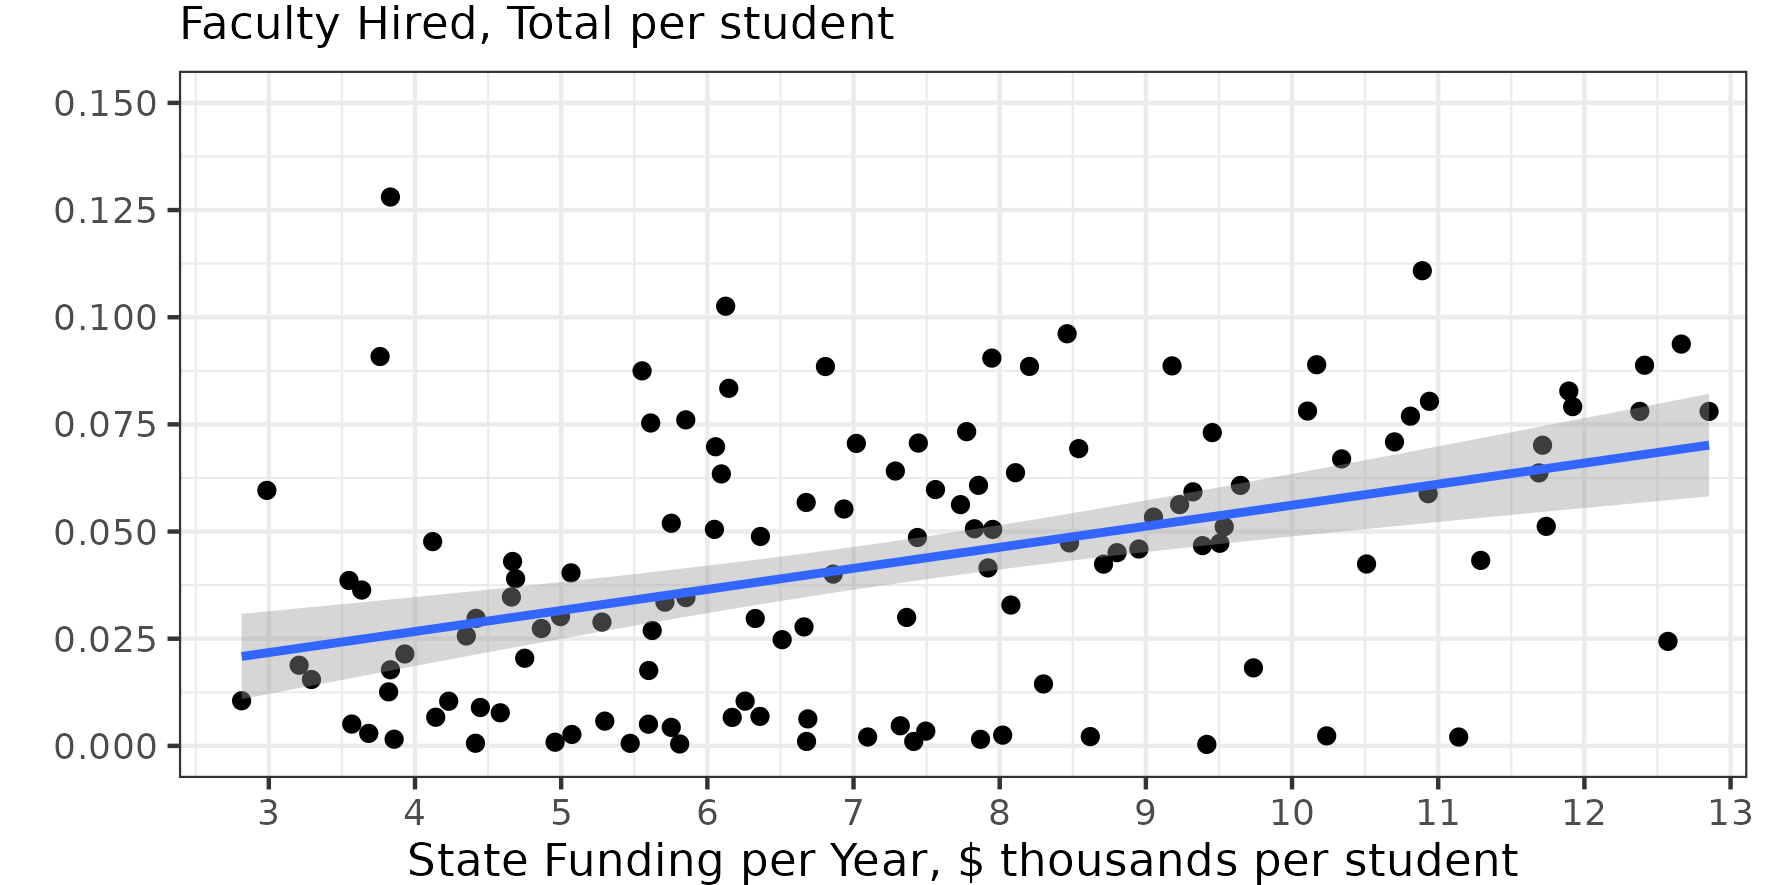
\includegraphics[width=0.8\textwidth]{figures/hiring-correlation.png}
    \label{fig:hiring-correlation.png}
\end{figure}

Universities with more state funding (for the entire decade) hired more professors (\autoref{fig:hiring-correlation.png}).
Similarly, the funding shock instrument identifies that an increase in 10\% state funding at an individual university leads to 13 more faculty hires on average across the decade 2011--2021 (see \autoref{tab:hiring-shock-reg}).\footnote{
    These results were produced by integrating the total count of faculty hires for 2010--2021 for the top-ranked 180 US universities with a sum of the funding variables, and then estimating the models specified in \autoref{sec:iv-model-uni}.
    There were no observable differences in the hiring rate of ale vs female faculty.
    See \autoref{sec:appendix-hiring} for further details.
}
It is clear that public universities' hiring is negatively impacted by falls in state funding, even using highly aggregated data for a total count of hiring across an entire decade.
While this analysis strengthens the case negative effects on hiring plays, it is crude for measuring exact magnitudes for the effect on faculty hiring; I leave it to further research to delve deeper into the magnitudes that hiring plays as the primary causal mediator for the effects of falls in state funding on faculty composition at public universities.
